% Name: LSTM cell
% Description: A long short-term memory cell: the forget, input, and output gates, the candidate, and the cell state running along the top.
% Tags: LSTM, recurrent network, gates, sequence model

\usetikzlibrary{arrows.meta}

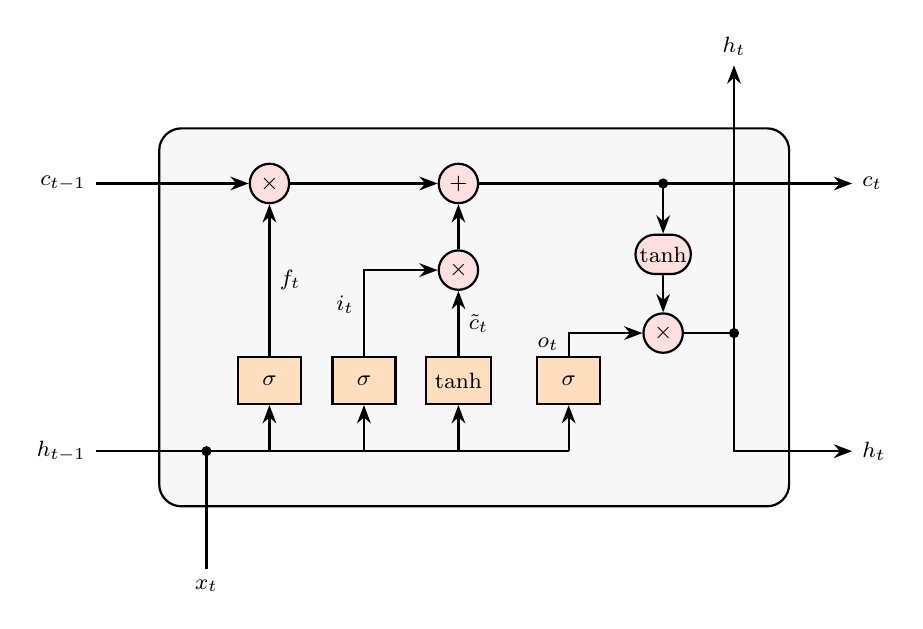
\begin{tikzpicture}[>={Stealth}, thick, every node/.style={font=\footnotesize},
    gate/.style={draw, fill=orange!25, minimum width=8mm, minimum height=6mm},
    op/.style={circle, draw, fill=red!12, inner sep=0pt, minimum size=5mm},
    dot/.style={circle, fill, inner sep=1.3pt}]
  \draw[rounded corners=8pt, fill=gray!6] (0,-0.3) rectangle (8,4.5);
  \node[gate] (f) at (1.4,1.3) {$\sigma$};
  \node[gate] (i) at (2.6,1.3) {$\sigma$};
  \node[gate] (g) at (3.8,1.3) {$\tanh$};
  \node[gate] (o) at (5.2,1.3) {$\sigma$};
  \node[op] (mf) at (1.4,3.8) {$\times$};
  \node[op] (mi) at (3.8,2.7) {$\times$};
  \node[op] (add) at (3.8,3.8) {$+$};
  \node[op, rounded corners=2.5mm, rectangle, inner sep=1.5pt] (th) at (6.4,2.9) {$\tanh$};
  \node[op] (mo) at (6.4,1.9) {$\times$};
  % The cell state along the top.
  \draw[->] (-0.8,3.8) node[left] {$c_{t-1}$} -- (mf);
  \draw[->] (mf) -- (add);
  \draw[->] (add) -- (8.8,3.8) node[right] {$c_t$};
  \draw[->] (6.4,3.8) node[dot] {} -- (th);
  \draw[->] (th) -- (mo);
  % The previous output and the input, shared by the four layers.
  \draw (-0.8,0.4) node[left] {$h_{t-1}$} -- (5.2,0.4);
  \draw (0.6,-1.1) node[below] {$x_t$} -- (0.6,0.4) node[dot] {};
  \foreach \n in {f, i, g, o} \draw[->] (\n |- 0,0.4) -- (\n);
  \draw[->] (f) -- node[right] {$f_t$} (mf);
  \draw[->] (i) |- node[pos=0.3, left] {$i_t$} (mi);
  \draw[->] (g) -- node[right] {$\tilde{c}_t$} (mi);
  \draw[->] (mi) -- (add);
  \draw[->] (o) |- node[pos=0.25, left] {$o_t$} (mo);
  \draw[->] (mo) -| (7.3,0.4) -- (8.8,0.4) node[right] {$h_t$};
  \draw[->] (7.3,1.9) node[dot] {} -- (7.3,5.3) node[above] {$h_t$};
\end{tikzpicture}
